\begin{figure*}[t]
  \centering
  % 从完整可编辑七方法图中无损裁取正文关键方法列；完整版本见附录。
  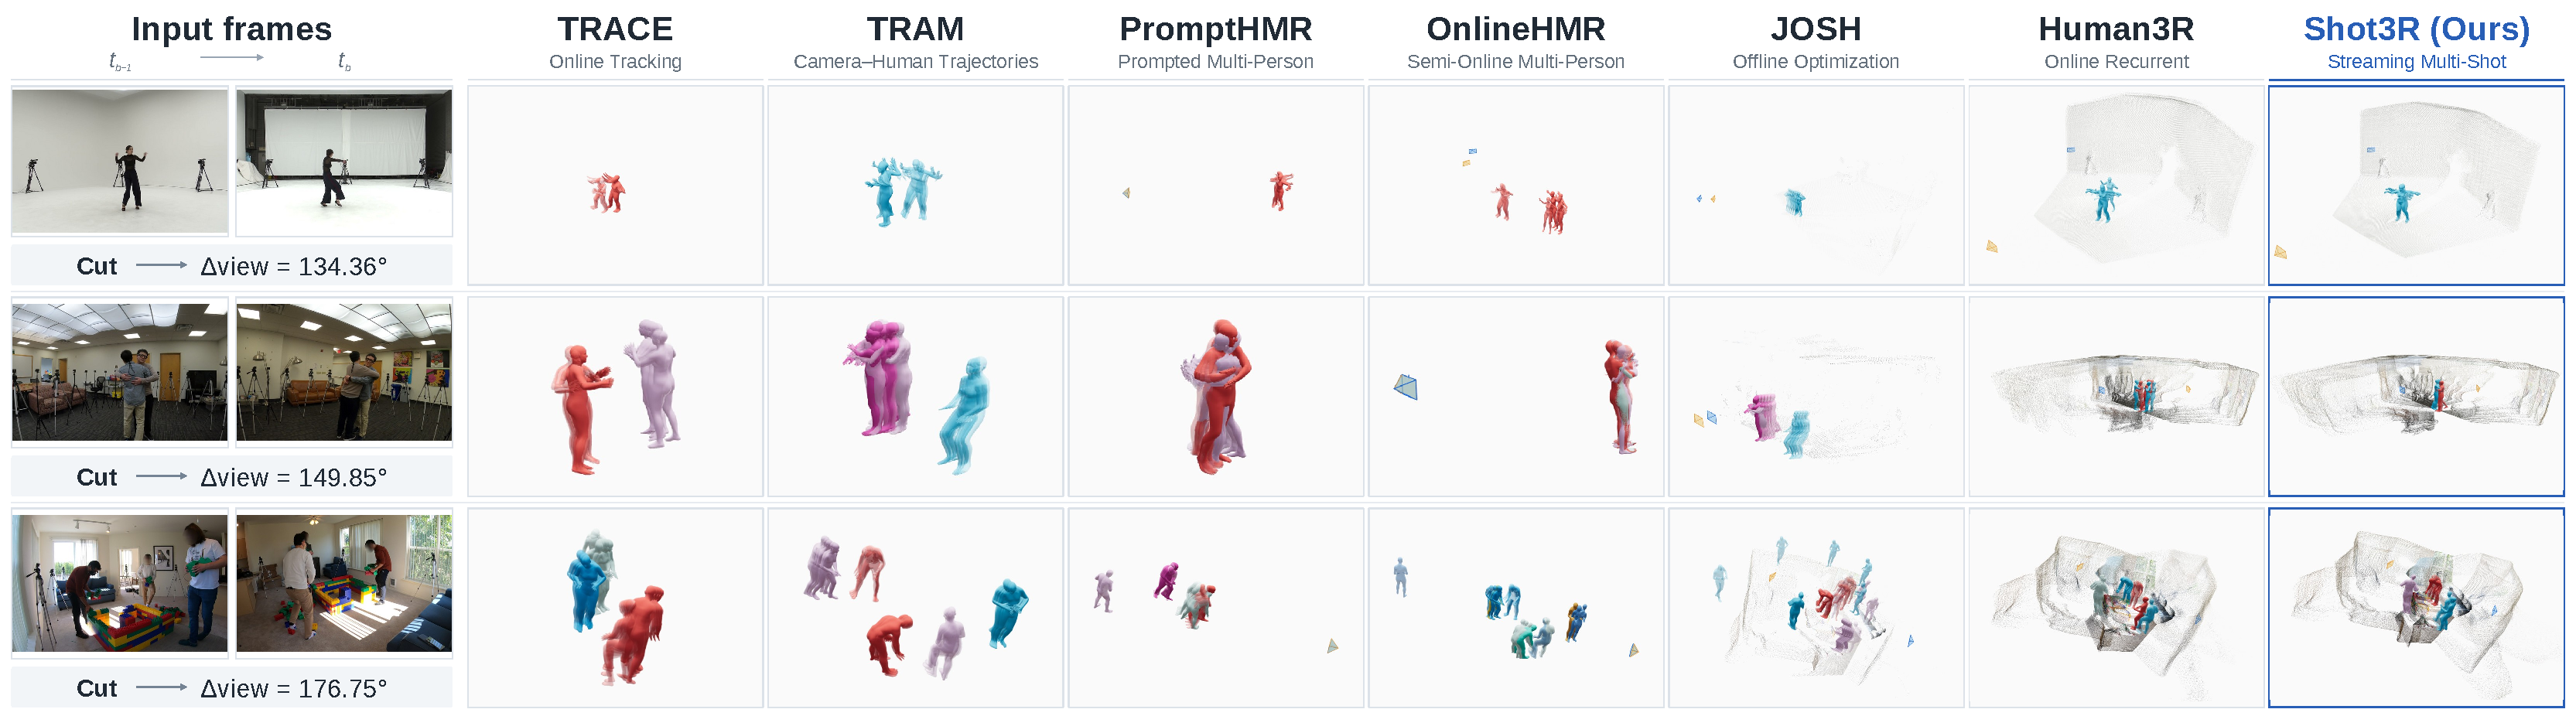
\includegraphics[height=0.415\textwidth,trim=0pt 0pt 1315pt 0pt,clip]{figures/Shot3R_qualitative_comparison.pdf}\hspace{-1.2mm}%
  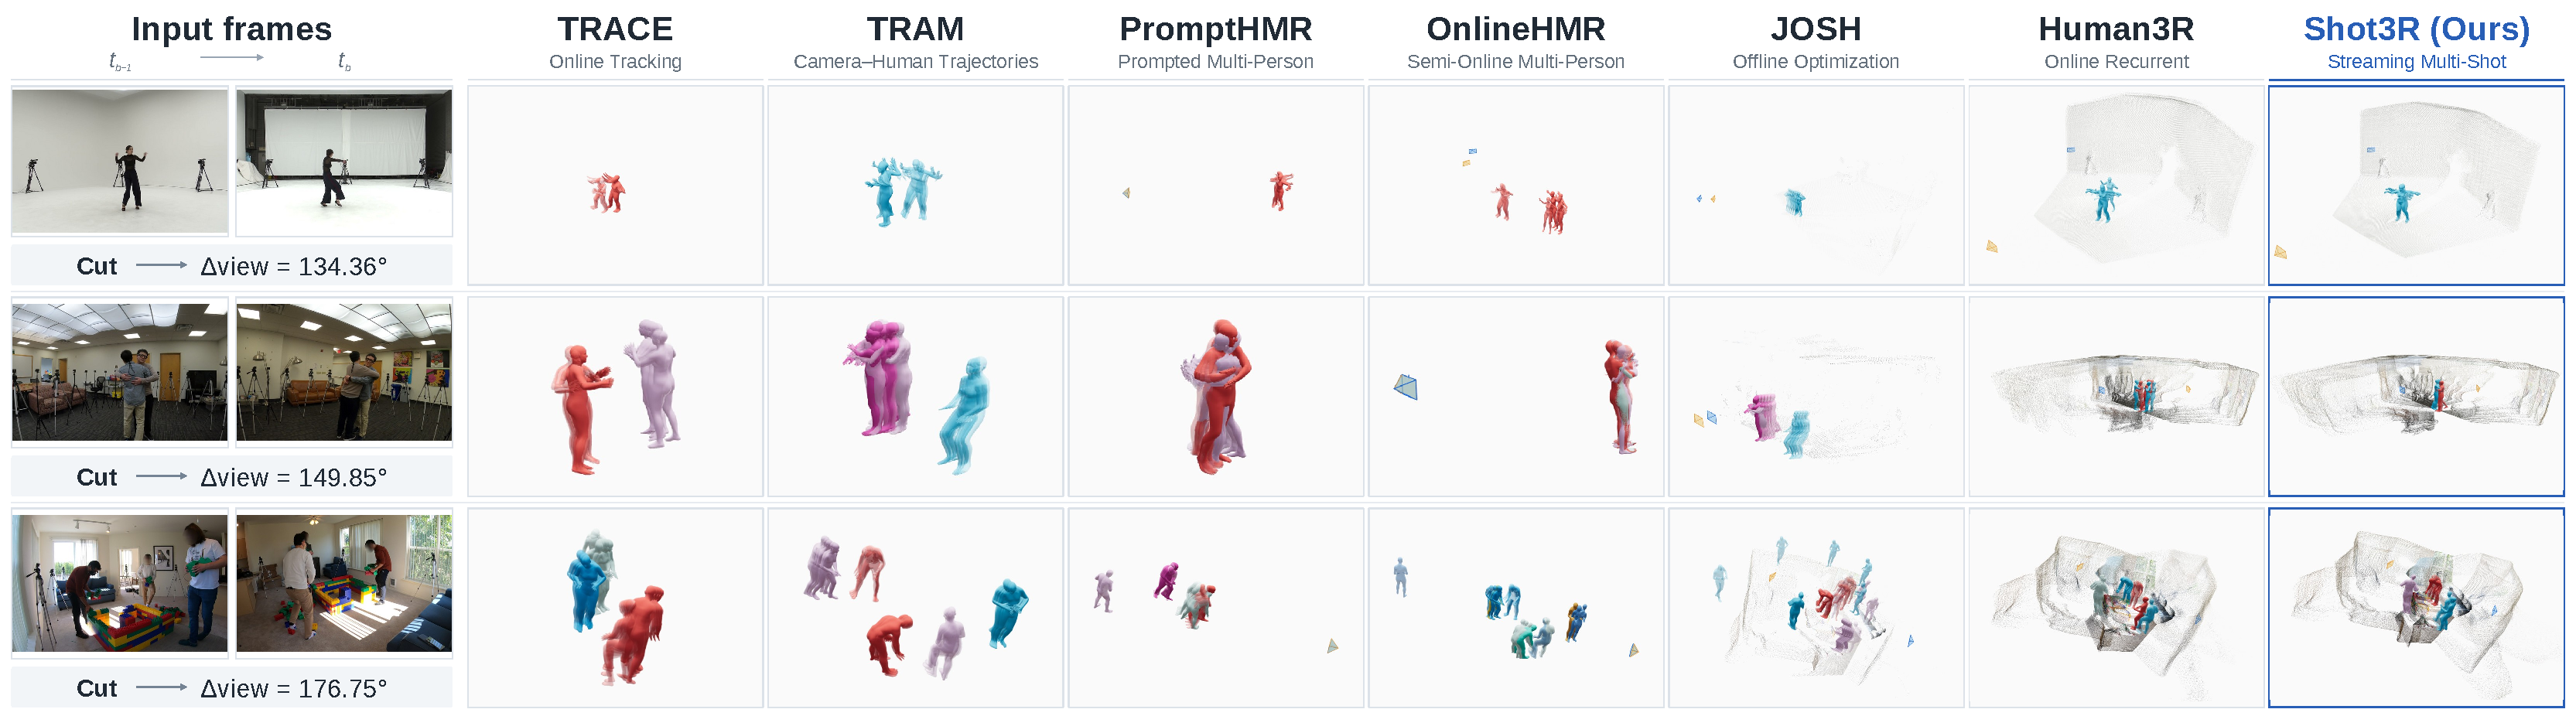
\includegraphics[height=0.415\textwidth,trim=845pt 0pt 560pt 0pt,clip]{figures/Shot3R_qualitative_comparison.pdf}\hspace{-1.2mm}%
  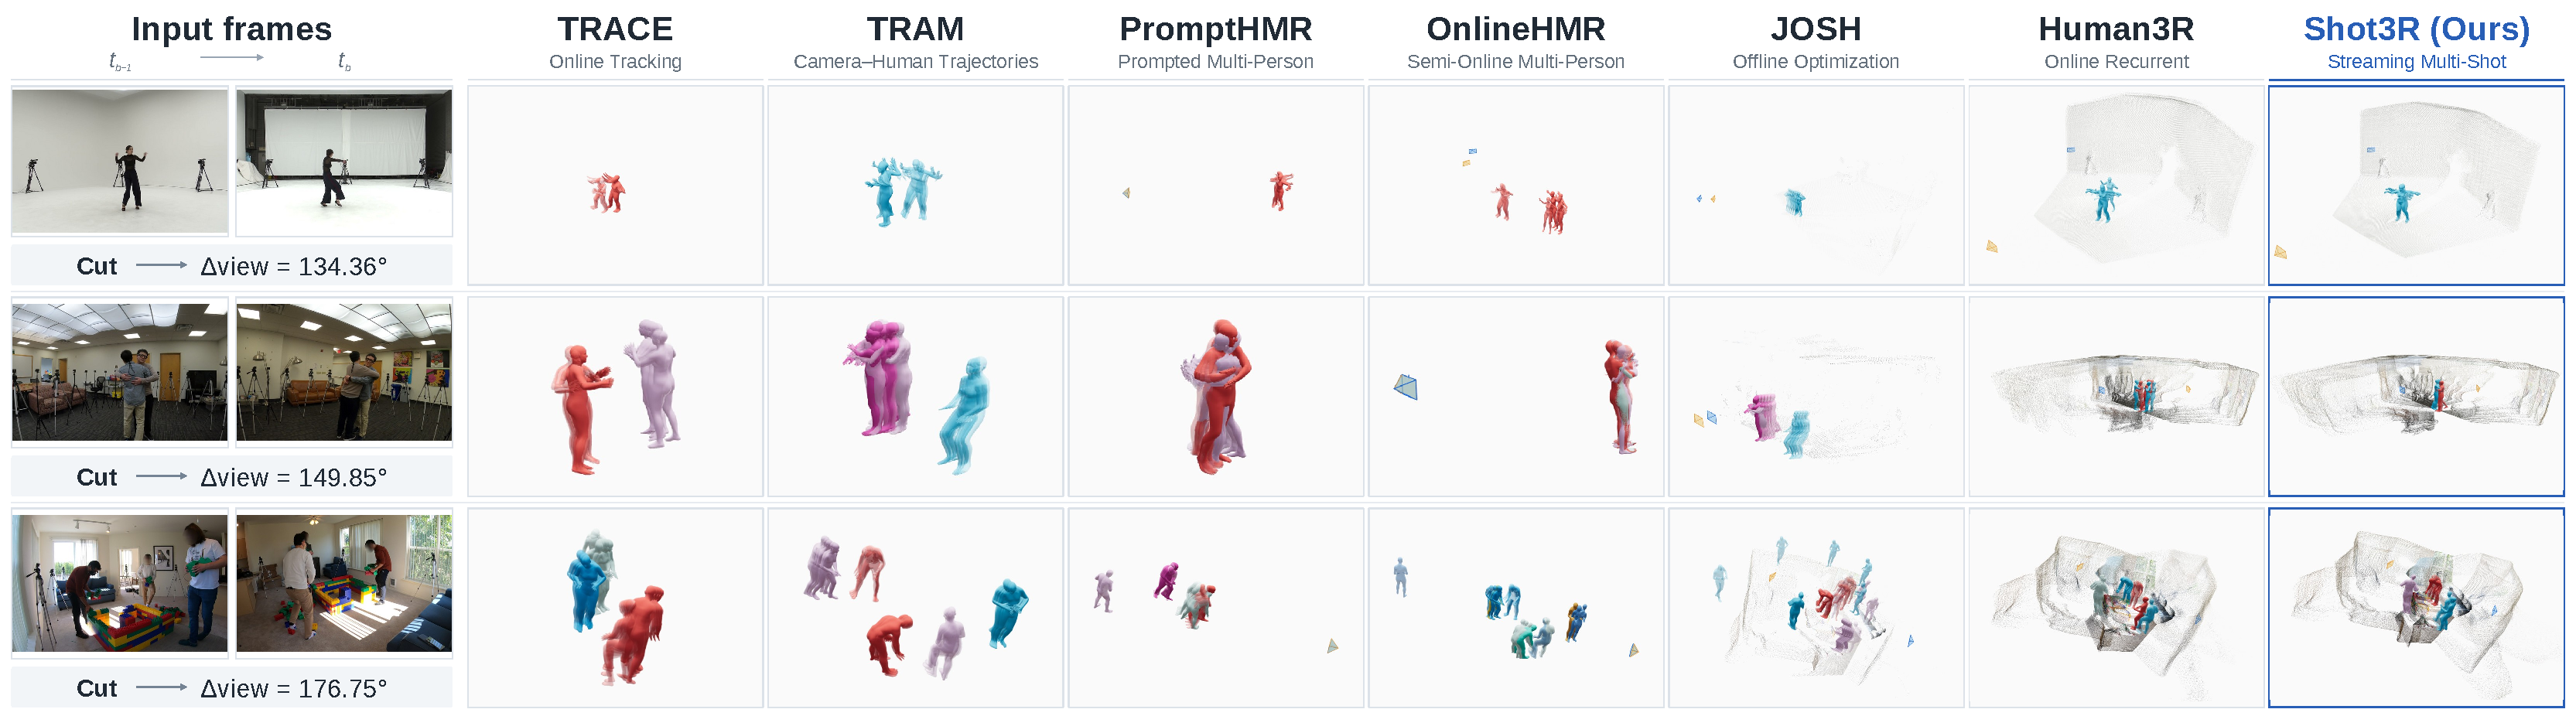
\includegraphics[height=0.415\textwidth,trim=1034pt 0pt 374pt 0pt,clip]{figures/Shot3R_qualitative_comparison.pdf}\hspace{-1.2mm}%
  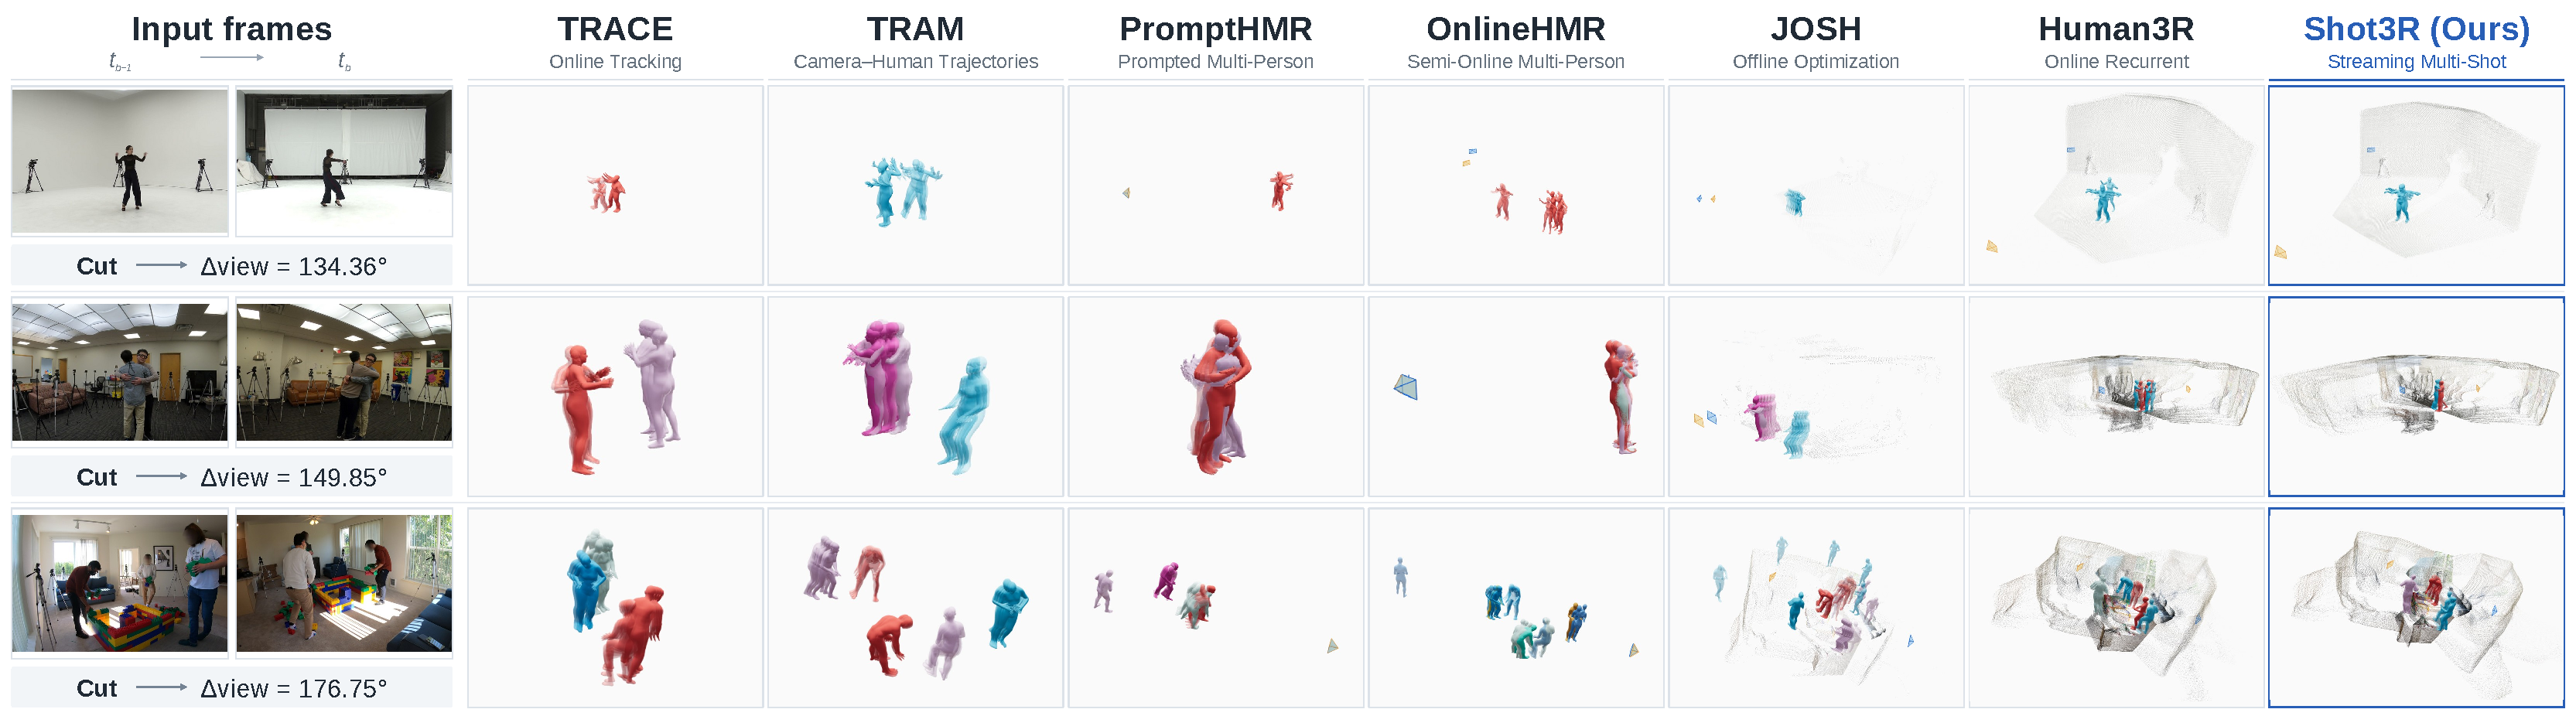
\includegraphics[height=0.415\textwidth,trim=1220pt 0pt 188pt 0pt,clip]{figures/Shot3R_qualitative_comparison.pdf}\hspace{-1.2mm}%
  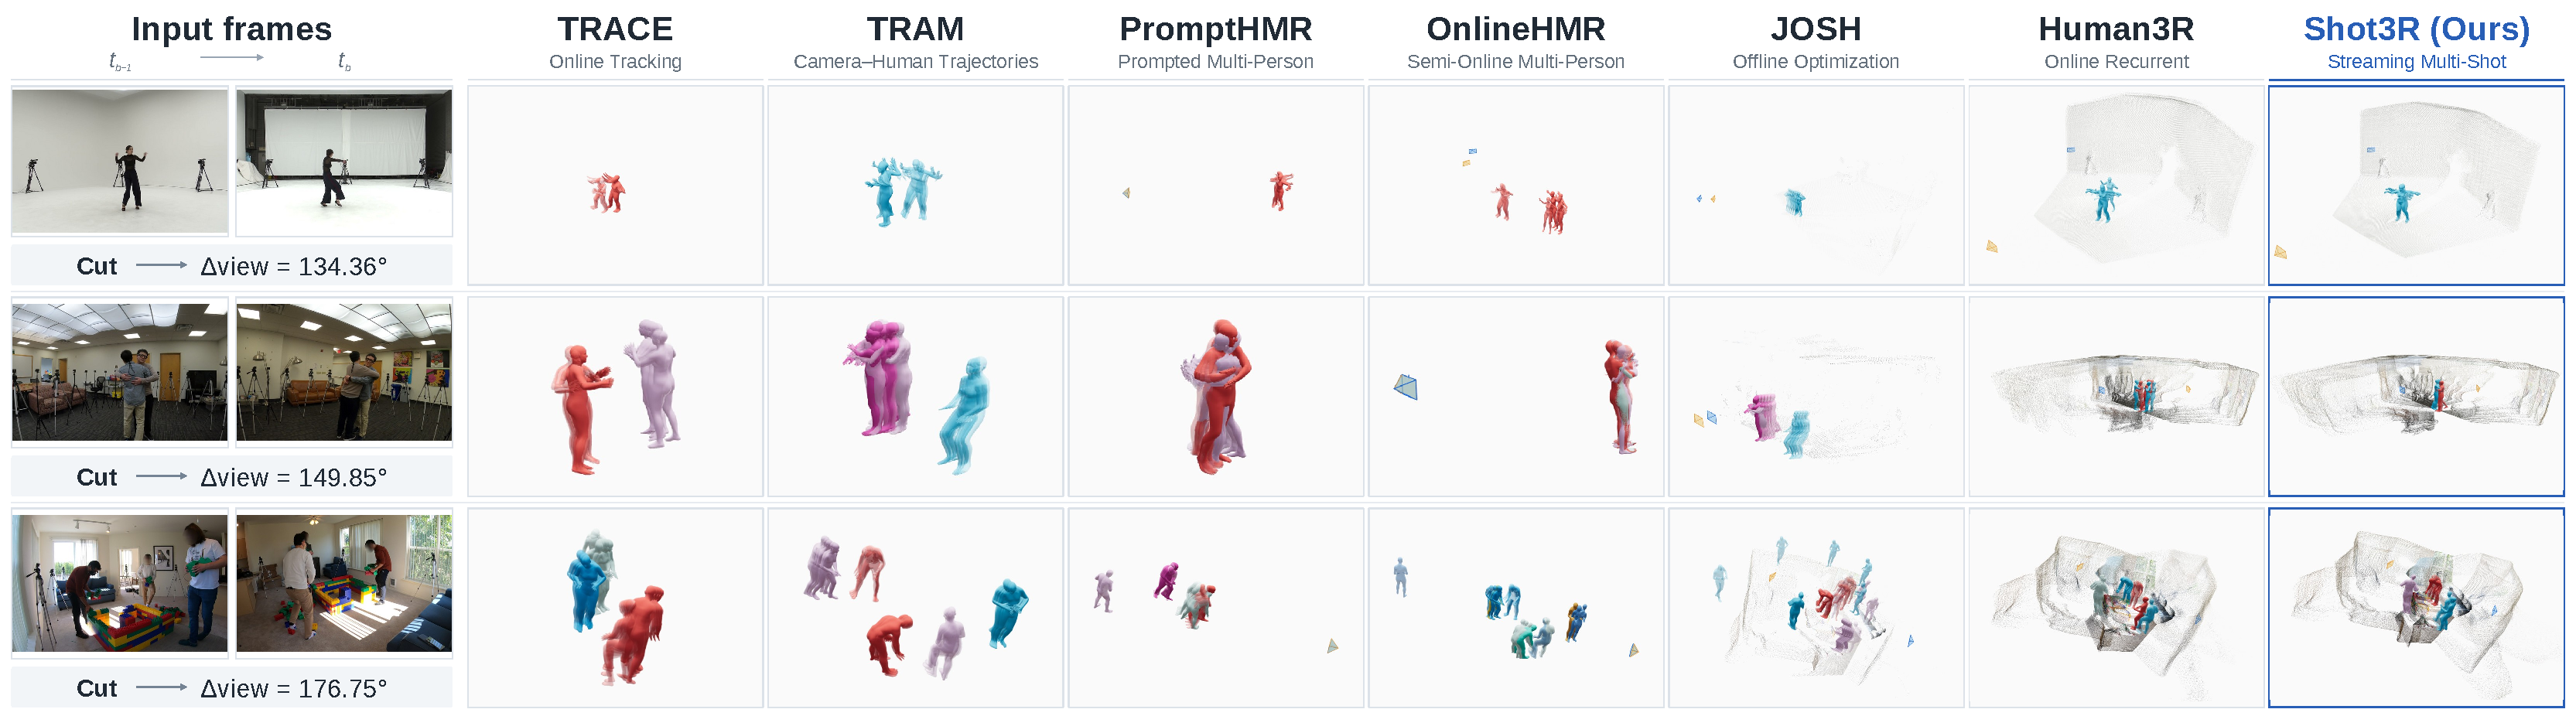
\includegraphics[height=0.415\textwidth,trim=1407pt 0pt 0pt 0pt,clip]{figures/Shot3R_qualitative_comparison.pdf}
  % 中文图注：跨镜头切换的关键定性比较。每一行首先展示切换前后的输入，随后是半在线、离线、在线递归基线与本文结果。
  % 三个视角变化从上到下为134.36、149.85和176.75度。Shot3R维持更连贯的相机—人体布局；各方法可用的场景输出一并显示。
  \caption{\textbf{Key qualitative comparisons across shot transitions.}
  Inputs before and after each transition are followed by OnlineHMR, JOSH,
  \humanthree{}, and \method{}. Viewpoint changes are $134.36^\circ$,
  $149.85^\circ$, and $176.75^\circ$ from top to bottom. \method{} maintains a
  more coherent camera--human layout; scene geometry is shown where available.
  The complete seven-method view is in Appendix~\ref{app:qualitative-full}.}
  \label{fig:qualitative-comparison}
\end{figure*}
